%
\begin{figure}
  \centering
  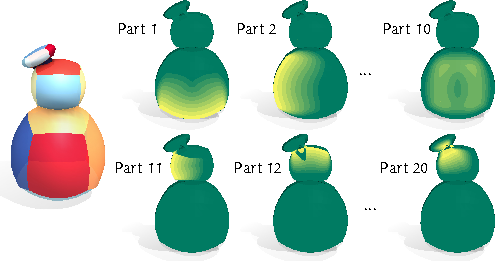
\includegraphics[width=3.33in]{figures/distance_weight_puft.pdf}
  \caption{Our distance weights decay smoothly from 1.0 (yellow) to 0.0 (green) when moving away from its closest surface. Here we visualize the distribution of the distance weights (with cutoff distance 5.0) corresponding to each part.   
  }
  \label{fig:distance_weight_puft}
  \vspace{-5pt}
\end{figure} 
%
%
\begin{figure}
  \centering
  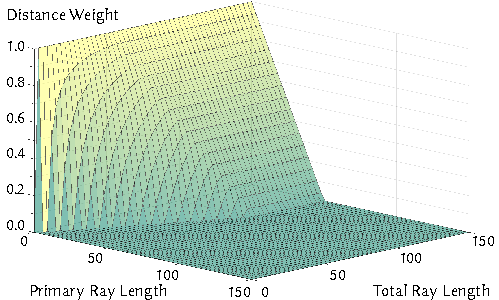
\includegraphics[width=3.33in]{figures/plot_distance_weight.pdf}
  \caption{We plot the distance weight with respect to the primary and total ray length. Here the cutoff distance is 50.
  }
  \label{fig:plot_distance_weight}
  \vspace{-5pt}
\end{figure} 
%